\documentclass{beamer}
\usetheme{Copenhagen}
\usepackage{listings}
\usepackage{minted}
\usepackage{graphicx}
\usepackage{subfig}
\usepackage{macros}

\title{Implémentation du protocole CRS d'échange de clefs à base d'isogénies }
\author{Hugo Nartz, Cl\'ement Jacquot}
\date{16 F\'evrier 2022}

%Page number
\expandafter\def\expandafter\insertshorttitle\expandafter{%
  \insertshorttitle\hfill%
  \insertframenumber\,/\,\inserttotalframenumber}

%%%%%%%%%%%%%%%%%%%%%%%%%%%%%%%%%%%%%%%%%%%%%%%%%%%%%%
%% Titlepage
%%%%%%%%%%%%%%%%%%%%%%%%%%%%%%%%%%%%%%%%%%%%%%%%%%%%%%
\begin{document}
\begin{frame}
  \titlepage
\begin{figure}[h]
\centering
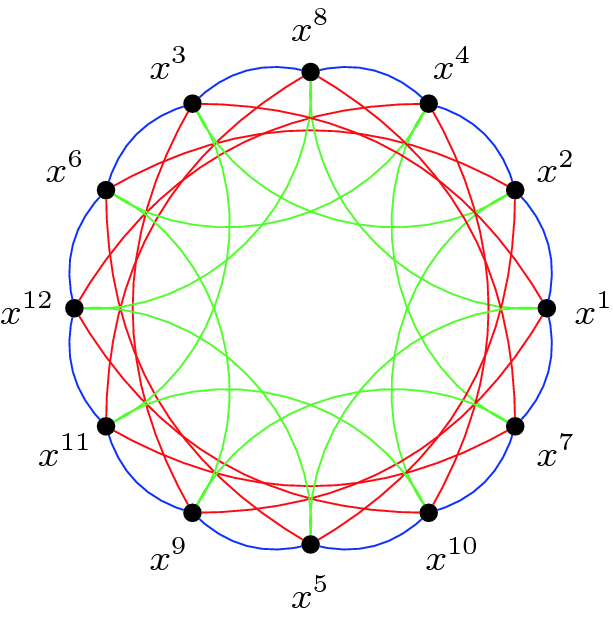
\includegraphics[scale=0.13]{../figs/isoGraph}
\end{figure}
\end{frame}

%%%%%%%%%%%%%%%%%%%%%%%%%%%%%%%%%%%%%%%%%%%%%%%%%%%%%%
%% Toc
%%%%%%%%%%%%%%%%%%%%%%%%%%%%%%%%%%%%%%%%%%%%%%%%%%%%%%
\begin{frame}{}
  \tableofcontents
\end{frame}

\section{Le protocol CRS}

%%%%%%%%%%%%%%%%%%%%%%%%%%%%%%%%%%%%%%%%%%%%%%%%%%%%%%
%% Parametres
%%%%%%%%%%%%%%%%%%%%%%%%%%%%%%%%%%%%%%%%%%%%%%%%%%%%%%
\begin{frame}{Param\`etres globaux}
	Corps de base:
	\[
		\mathbb{F}_p \text{ avec } p\sim 2^{512}.
	\]
	Courbe de base avec de bonnes propri\'et\'es:
	\[
		E: Y^2 = X^3 + AX^2 + X  \text{ o\`u } A\in  \mathbb{F}_p.
	\]
	Notamment $\# E(\FFp) = 3\cdot 5\cdot 7\cdot 11 \cdot 13\cdot 17\cdots$
\end{frame}

%%%%%%%%%%%%%%%%%%%%%%%%%%%%%%%%%%%%%%%%%%%%%%%%%%%%%%
%% Isogenies
%%%%%%%%%%%%%%%%%%%%%%%%%%%%%%%%%%%%%%%%%%%%%%%%%%%%%%
\begin{frame}{Isog\'enies et Frobenius}
	\begin{itemize}
		\item  $l$: petit diviseur premier de $\#E(\FFp)$ co-premier \`a $p$.
		\item Pour  tout $P\in E(\FFp)[l]$ il existe une unique $l$-isog\'enie
	\[
		\phi: E\rightarrow E/<P>
	\]
	telle que $\ker\phi = <P>$.
\item Pour certains $l$ (\textit{Elkies primes}), le Frobenius
		\[
			\pi: (x, y)\in E[l]\mapsto (x^p, y^p)\in E[l]
		\]
	a deux valeurs propres $\lambda$ et $\mu$.
\item $E[l]$ est somme de deux sous-espaces propres de cardinaux $l$: deux isog\'enies associ\'ees.
	\end{itemize}
\end{frame}

%%%%%%%%%%%%%%%%%%%%%%%%%%%%%%%%%%%%%%%%%%%%%%%%%%%%%%
%% Graphes
%%%%%%%%%%%%%%%%%%%%%%%%%%%%%%%%%%%%%%%%%%%%%%%%%%%%%%
\begin{frame}{Graphes d'isog\'enies}
	\begin{itemize}
		\item Deux $l$-isog\'enies par courbe: deux directions ($\lambda$ et $\mu$).
		\item Isog\'enie \textit{duale} de degr\'e $l$ ($\dashrightarrow$): pour revenir en arri\`ere.
		\item Conservation des propri\'et\'es dans la composante connexe
	\end{itemize}
	 \vspace*{0.2cm}
	$\rightarrow$ Pour chaque $l$ (Elkies): un cycle dont les sommets sont des courbes elliptiques et les ar\^etes des isog\'enies.
	 \vspace*{0.2cm}
	\begin{center}
		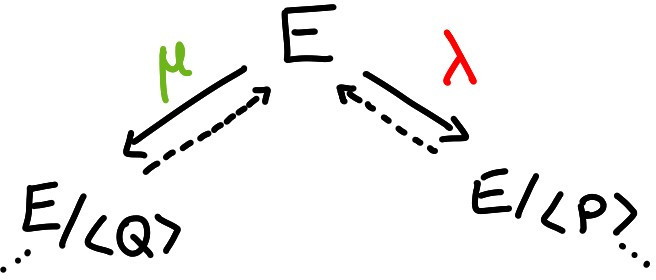
\includegraphics[scale=0.2]{../figs/Cycle}
	\end{center}
	$\rightarrow$ Les pas dans le graphe commutent par rapport aux différents $l$.
\end{frame}

%%%%%%%%%%%%%%%%%%%%%%%%%%%%%%%%%%%%%%%%%%%%%%%%%%%%%%
%% Echange de clefs
%%%%%%%%%%%%%%%%%%%%%%%%%%%%%%%%%%%%%%%%%%%%%%%%%%%%%%
\begin{frame}{L'\'echange de clefs}
	\begin{itemize}
		\item Clef priv\'ee $s$: nombre de pas (al\'eatoire) pour chaque $l$.
		\item Clef publique: marche suivant les pas de la clef secr\`ete $s\curvearrowright E$.
	\end{itemize}
	 %\vspace*{0.2cm}
\begin{center}
	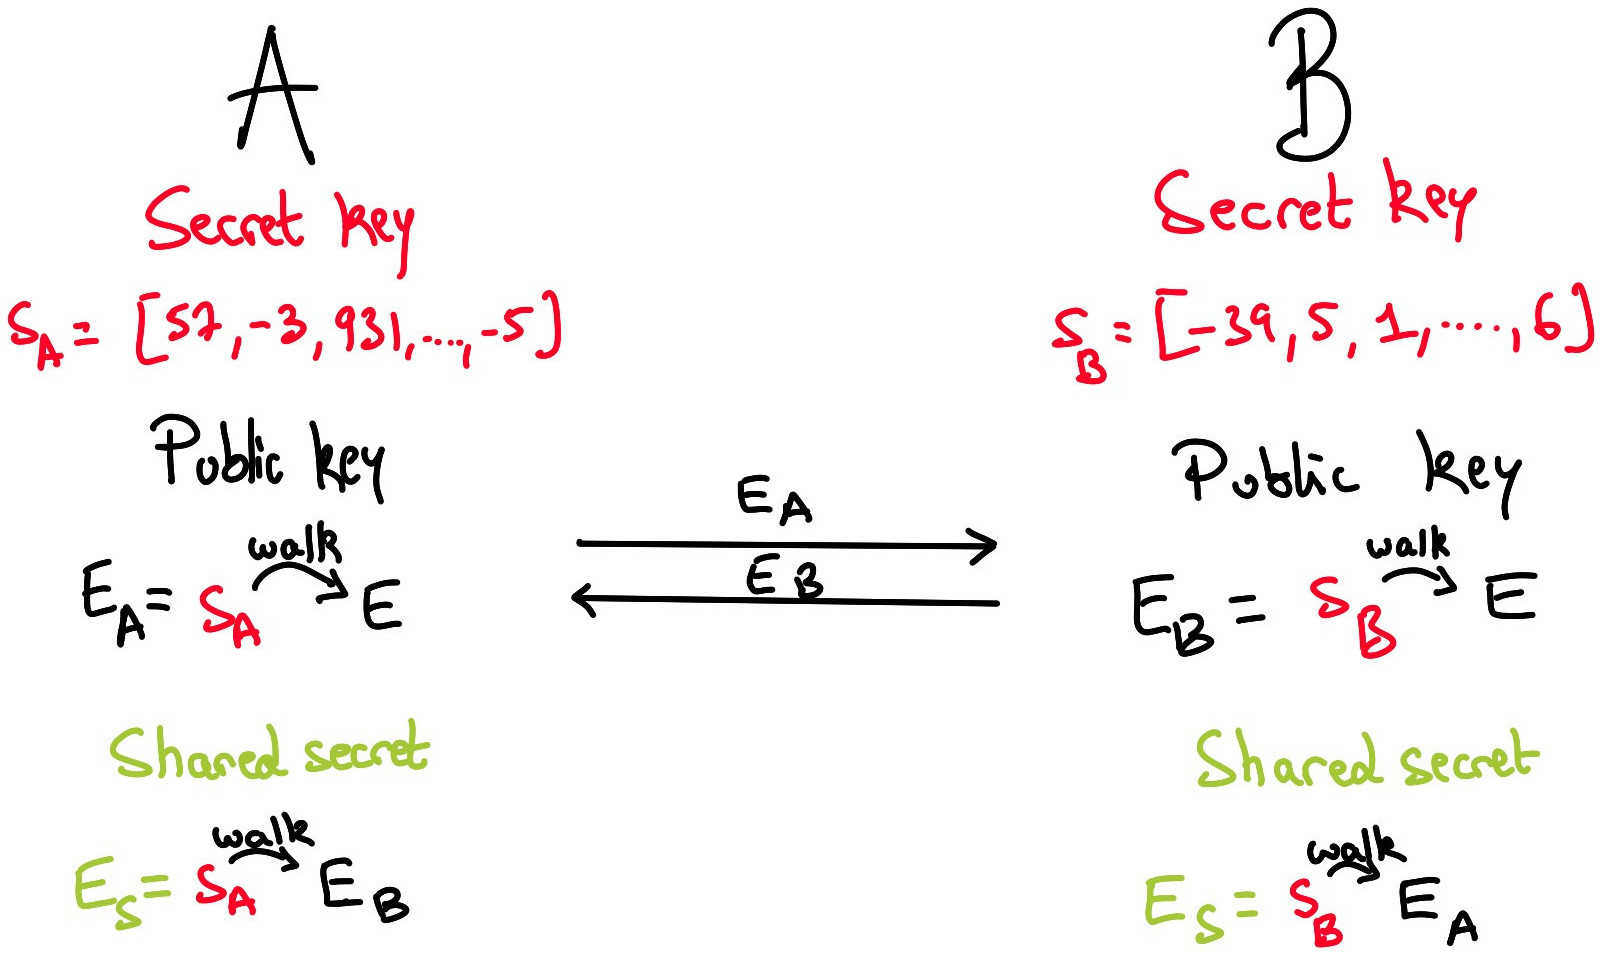
\includegraphics[scale=0.2]{../figs/DH}
\end{center}
\end{frame}

\section{Algorithmes}
%%%%%%%%%%%%%%%%%%%%%%%%%%%%%%%%%%%%%%%%%%%%%%%%%%%%%%
%% Torsion
%%%%%%%%%%%%%%%%%%%%%%%%%%%%%%%%%%%%%%%%%%%%%%%%%%%%%%
\begin{frame}{Points de $l$-torsion}
	On cherche $P\in E(\FFq)[l] = \ker\phi$. Posons $C = \#E(\FFq) / l$.
	\begin{itemize}
		\item Soit $Q\in E(\FFq)$ al\'eatoire.
		\item Si $P := C\cdot Q \neq O$, on a gagn\'e.
		\item Sinon on tire un autre $Q$.
	\end{itemize}
	Si $\#E(\FFq) = l \cdot p_1 ^{f_1}\cdots p_n^{f_n}$ avec $l\wedge p_i = 1$,
	\begin{align*}
		Q &= (e_0, e_1, \cdots, e_n)\in \Z_{l}\times \Z_{p_1^{f_1}}\times \Z_{p_n^{f_n}},\\
		C\cdot Q &= (\kappa e_0, 0, \cdots, 0) \text{ pour } \kappa\in \FF_l^{*}.
	\end{align*}
	Le point $C\cdot Q$ convient avec probabilit\'e $1-1/l$.
\end{frame}

%%%%%%%%%%%%%%%%%%%%%%%%%%%%%%%%%%%%%%%%%%%%%%%%%%%%%%
%% Montgomery Arithmetic
%%%%%%%%%%%%%%%%%%%%%%%%%%%%%%%%%%%%%%%%%%%%%%%%%%%%%%
\newcommand{\x}{\textbf{x}}
\begin{frame}{Arithmétique de Montgomery}
	\begin{itemize}
		\item{ Courbe de Montgomery $E_{A,B} : By^2 = x^3+Ax^2 + x$}
		\item{ $\x\colon (X:Y:Z) \in E_{A,B} \mapsto (X:Z) \in \mathbb{P}^1$}
		\item{La loi de $E_{A,B}$ induit par {\x} une loi sur $\mathbb{P}^1$}
		\item[Prop.]{$P,Q\in E$\\ \hspace{-20pt}
			Si $P\neq Q$ alors\\
			{\small$\left\{\begin{array}{l}
					X_{P+Q} = Z_{P-Q}[(X_P-Z_P)(X_Q+Z_Q) + (X_P+Z_P)(X_Q-Z_Q)]^2\\
					Z_{P+Q} = X_{P-Q}[(X_P-Z_P)(X_Q+Z_Q) - (X_P+Z_P)(X_Q-Z_Q)]^2
				\end{array}\right.$}\\ \hspace{-20pt}
			Si $P=Q$ alors\\
			{\small$\left\{\begin{array}{l}
					X_{[2]P}=(X_P + Z_P)^2(X_P - Z_P)^2 \\
					Z_{[2]P}=(4 X_P Z_P)[(X_P - Z_P)^2 + \frac{A+2}{4}(4 X_P Z_P)]
				\end{array}\right.$}}
\end{itemize}\end{frame}

\begin{frame}{Arithmétique de Montgomery}
	\begin{itemize}
		\item{ Courbe de Montgomery $E_{A,B} : By^2 = x^3+Ax^2 + x$}
		\item{ $\x\colon (X:Y:Z) \in E_{A,B} \mapsto (X:Z) \in \mathbb{P}^1$}
		\item{La loi de $E_{A,B}$ induit par {\x} une loi sur $\mathbb{P}^1$}
		\item{On remonte à $E_{A,B}$ en remarquant que $\x(P)=\x(Q)\Leftrightarrow P=\pm Q$}
		\item{ $\x(P)+\x(Q)$ détermine $\lbrace\x(P \pm Q)\rbrace$}
		\item{xADD : $(\x(P),\x(Q), \x(P-Q)) \mapsto \x(P+Q)$}
		\item{xDBL : $\x(P) \mapsto \x(2P)$}
	\end{itemize}
\end{frame}

%%%%%%%%%%%%%%%%%%%%%%%%%%%%%%%%%%%%%%%%%%%%%%%%%%%%%%
%% Montgomery Ladder
%%%%%%%%%%%%%%%%%%%%%%%%%%%%%%%%%%%%%%%%%%%%%%%%%%%%%%
\begin{frame}[fragile]{Montgomery Ladder pseudocode}
	\small	Entrées : $P, k = \sum_{i=0}^{l-1}k_i 2^i$ avec $k_{l-1}=1$\\
	Sortie : $kP$
\begin{minted}[linenos, mathescape=true,fontsize=\footnotesize]{c}
P0 = P
P1 = xDBL(P)
for(int i=l-2; i>=0, i--) {
  if(k[i]==0){
    P1 = xADD(P0, P1, P)
    P0 = xDBL(P0)
  }
  else{
    P0 = xADD(P0, P1, P)
    P1 = xDBL(P1)
  }
}
return P0
\end{minted}
Invariants: $P1 = P0+P$ et après $i$ itérations,
$\begin{array}{l}P0 = \lfloor k/2^i\rfloor P \\ P1 = \lfloor k/2^i + 1\rfloor P\end{array}$
\end{frame}

%%%%%%%%%%%%%%%%%%%%%%%%%%%%%%%%%%%%%%%%%%%%%%%%%%%%%%
%% Vélu step
%%%%%%%%%%%%%%%%%%%%%%%%%%%%%%%%%%%%%%%%%%%%%%%%%%%%%%
\begin{frame}[fragile]{Vélu-step}
\begin{itemize}
	\item Donné : un point $P$ de l-torsion.
	\item But : effectuer un pas sur le graphe d'isogénies.
	\item[Prop.]{$\phi:E_A\rightarrow E_{A'}$ isogénie de noyau $\langle P \rangle$.\\
		On a alors $\boxed{A'=2\frac{1+d}{1-d}}$ où\\
		\[d = \left(\frac{A-2}{A+2}\right)^l \left( \frac{h_S(1)}{h_S(-1)}\right)^8 \text{ , et}\]
			\[h_S(X) = \prod_{s\in S}(X-\x([s]P))\text{, avec }S=\{1,3, \ldots, l-2\}\]}
\end{itemize}
\end{frame}

\begin{frame}[fragile]{Algorithme $\sqrt{}$\textit{-Velu}}
	\begin{itemize}
		\item{$h_S(X) = \prod_{s\in S}(X-\x([s]P))\text{, avec }S=\{1,3, \ldots, l-2\}$}
		\item[Idée.] {Ecrire $S=(I\pm J) \cup K$} avec $\sqrt{l/2}\simeq \#I \simeq \#J \simeq \#K$
		\item{$h_{I\pm J} = h_{I+J} h_{I-J}$}
		\item{$\x(P), \x(Q), \x(P+Q), \x(P-Q)$ sont fondamentalement reliés.}
		\item{On exprime $h_{I\pm J}=\text{Res}(h_I, R_J)$ où $R_J\in\FFp[X]$}
		\item{Les racines de $h_I$ étant connues, ce calcul se ramène à une multi-évaluation
			\[\text{Res}(h_I, R_J)=\prod_{i\in I}R_J(\x([i]P))\]}
	\end{itemize}
\end{frame}

%%%%%%%%%%%%%%%%%%%%%%%%%%%%%%%%%%%%%%%%%%%%%%%%%%%%%%
%% Multi-evaluation
%%%%%%%%%%%%%%%%%%%%%%%%%%%%%%%%%%%%%%%%%%%%%%%%%%%%%%
\begin{frame}{Multi-evaluation}
	\begin{itemize}
		\item Probl\`eme:  \'evaluer $P\in\FFq[X]$ en $\alpha_1,\cdots, \alpha_n$.
		\item Equivalent \`a $P$ mod $(X-\alpha_i)$.
	\end{itemize}
	Exemple pour $n=4$: on construit par le bas
	\begin{center}
		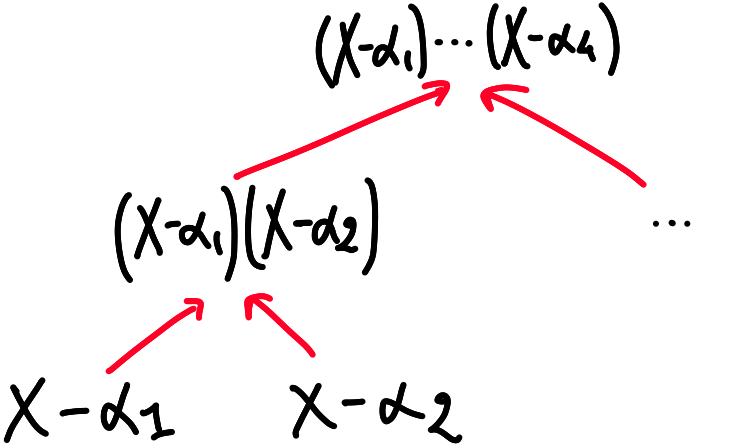
\includegraphics[scale=0.2]{../figs/tree}
	\end{center}
	Puis on r\'eduit $P$ en descendant.\\
	Complexit\'e: $\mathbf{M}(n)\log n$ si $\text{deg}(P) \sim n$.
\end{frame}

\section*{Conclusion}
\begin{frame}
\end{frame}

%%%%%%%%%%%%%%%%%%%%%%%%%%%%%%%%%%%%%%%%%%%%%%%%%%%%%%
%% Démo formules Montgomery
%%%%%%%%%%%%%%%%%%%%%%%%%%%%%%%%%%%%%%%%%%%%%%%%%%%%%%
\begin{frame}{Formules d'additions affine}\small
	Soient $P=(x_P,y_P), Q=(x_Q,y_Q) \in E_{A,B}$ avec $x_P \neq x_Q$ et $x_P x_Q \neq 0$.
	Notons $P+Q=(x_{P+Q},y_{P+Q})$ et $P-Q=(x_{P-Q},y_{P-Q})$. Alors $x_{P+Q}$ satisfait
	\[\begin{aligned}
		x_{P+Q}	&= B[(y_P - y_Q)/(x_P-x_Q)]^2 - A - x_P - x_Q \\
		&= \frac{1}{(x_P-x_Q)^2}( B(y_P - y_Q)^2 - (A + x_P + x_Q)(x_P - x_Q)^2) \\
		&= \frac{1}{(x_P-x_Q)^2}( -2B y_P y_Q + x_P x_Q (x_P + x_Q + 2A) + x_P + x_Q) \\
		&= \frac{B(x_Q y_P - x_P y_Q)^2}{x_P x_Q (x_P-x_Q)^2}
	\end{aligned}\]
	De même, $x_{P-Q} = \frac{B(x_Q y_P + x_P y_Q)^2}{x_P x_Q (x_P-x_Q)^2}$
	
	En multipliant ces équations, on obtient
	\[x_{P+Q} x_{P-Q} (x_P - x_Q)^2 = (x_p x_Q -1)^2\]
\end{frame}

\begin{frame}{Formules d'additions projectives}\small
	On passe en coordonnées projectives. En écrivant les quotients $x=X/Z$ pour chaque point en question,
	On vérifie alors que $\x(P+Q)=(X_{P+Q}:Z_{P+Q})$ avec \[X_{P+Q} = Z_{P-Q}(X_P X_Q - Z_P Z_Q)^2\]\[Z_{P+Q} = X_{P-Q}(X_P Z_Q - Z_P X_Q)^2\]
	Ces formules nécessitent 8 multiplications mais peuvent être réécrites en
	\[\begin{array}{l}
		X_{P+Q} = Z_{P-Q}[(X_P-Z_P)(X_Q+Z_Q) + (X_P+Z_P)(X_Q-Z_Q)]^2\\
		Z_{P+Q} = X_{P-Q}[(X_P-Z_P)(X_Q+Z_Q) - (X_P+Z_P)(X_Q-Z_Q)]^2
	\end{array}\]
	qui ne nécessitent plus que 6 multiplications.
\end{frame}

\end{document}
